\documentclass{article}
\usepackage[preprint]{neurips_2024}
\usepackage{graphicx} % Required for including graphics
\usepackage{hyperref} % Required for hyperlinks
\usepackage{float} % Required for positioning figures and tables at the correct location

\title{Neuromorphic Swarm Autonomy: Monocular Event-Based Swarm Navigation in Cluttered Environments}
\author{
    Amit Nativ \\ 
    Supervisor: Oren Gal \\
    \\
    Swarm \& AI Lab \\
    Hatter Department of Marine Technologies \\
    Leon H. Charney School of Marine Sciences \\
    University of Haifa \\
    \\
    \\
    April 1, 2024
}

\begin{document}

\maketitle

\begin{abstract}
\begin{enumerate}
    \item Event camera under canopy of trees
    \item Event camera in the wild
    \item Path planning
    \item Dodging dynamic obstacles
    \item Dodging dynamic obstacles in swarm formation
    \item RL with spiking nueral networks - spiking nueral networks for high speed control
    \item fuse mono RGB and event camera to improve obstacle avoidance in both high and low speeds. 
    \item \textbf{Use DeepSeek Group Relative Policy Optimization (GRPO) for SWARM???} 
    \item \textbf{Use event camera, snn, Neuromorphic chip for agile flight of drones in the wild with both dynamic and static obstacles}
    \item Adding a drone to the swarm, after the swarm formation is formed. the drones will reform to optimal formation.
    \item VLA for drone flight with SNN
    \item flightMare, MAVLAB benchmark, SNNtorch
    
\end{enumerate}
\end{abstract}

\section{Research Questions}
    \begin{enumerate}
        \item Event-based learning and control for UAVs using spiking neural networks.
        \item Event-based emerging swarm intelligence for UAVs.
        \item Implementation of SNN on neuromorphic hardware for UAVs.
        \item Dynamic obstacle avoidance of swarms using event-based cameras.
        \item swarm control in cluttered environments using event-based cameras.
        \item Event-based SNN for high-speed control of UAVs in the wild.
        \item Event-based SNN obstacle avoidance in swarms.
    \end{enumerate}
    
\section{Scaramuzza}
\begin{itemize}
    \item Low latency
    \item High temporal resolution
    \item Asynchronous data output
    \item High dynamic range
    \item Low power consumption
    \item Event camera measure changes in intensity - caused by motion or blinking light.
    \item You can control the senstivity of the camera.
    \item In contrast to normal camera, that outputs the intensity measurements in a constany frequency,
    \item However, in an event camera, each pixel will trigger an event regardless of other pixels, whenever there is a change 
    \item In intensity is detected on that pixel. This is a very low latency camera.
    \item 1MHz upper timer limit.
    \item \textbf{The price is still high, but like a Lidar, but companies are strarting to sell chepar event cameras
                    when Tthey are sold a s product (Samsung SmartThings vision)}
    \item \textbf{The price is exepecteed to reduce in the future, like it was with ToF cameras}
    \item Spiking neural network. Event cameras are very low power consumers. In robotics - that can increase flight time
    \item frame based cameras have a latency of ~30Hz or ~60Hz. For agile flight, in high speeds this is not enough.
            You can increase the frame rate, but than you will have a very high bandwidth. (You move on the bandwidth frame rate parabula) 
\end{itemize}

\textbf{Contrast sensitivity}

\textbf{The signal in continuous in the intensity (y) axis, and not on the temporal axis (x)}
    Can we integrate an event camera with a very simple normal camera to get human like vision system (sensitve to intensity + changes?)
    Super usefull for SLAM in high speed manuvers!!!!
\\
\\
Event camera allow SLAM at high speeds, with vaiations in light. even with minimal light (0.1 Lux - fullmoon)

\textbf{second school methods - Batch processing}
\\
reconstuct the events in batches
\begin{itemize}
    \item  Image stabliization vision only without the IMU or mechinal stablization
    \item The contrast, using contrast maximization algo, can be used for self supervised learning.
    \item Motion Segmentation
    \item Event camera + IMU + GPS
    \item Event camera + IMU + GPS + Lidar
    \item Event camera + IMU + GPS + Lidar + Normal camera


Combine event cameras with standard cameras. 
\item Event camera is a high pass filter - focuses on high changes in the Image
\item Standard camera can be viewed as low pass camera 
\item Scaramuzza - event camera + normal camera \textit{Low Latency Automotive Vision with Event Cameras, Nature, 2024}
\begin{itemize}
    \item They shown that using a 20fps camera plus an event camera can achive the same latency as a 5000fps camera, with bandwidth of 50fps, without compromising the accuracy.
\end{itemize}
    
\textbf{Neuromorphic sensors}
\textit{Synsense}

Spiking Neural Network - An approach using asynchorounous processing - SNN.
\end{itemize}

\section{How can this be used in Robotics}
\begin{itemize}
    \item Low-latency, High-Bandwidth Control.
    \item High-speed SLAM
    \item High-speed path planning
    \item High-speed obstacle avoidance
    \item High speed control commands
    \item Spiking Neural Network look promissing for high speed control
\end{itemize}
    
\textit{[1] Vitale et al., Event-driven Vision and Control for UAVs on a Neuromorphic Chip}
\\
\textit{[2] Sugimoto et al., Towards Low-Latency Hig-Bandwidth Control of Quadrotors using Event Cameras}
\\
\\
\textbf{Currently it only works on 1 axis. They try to do it on 6DOF}
\\
\textbf{Apple and Meta pulished over 100 patents on event cameras - at 2019}
\\
\textbf{2021 - Sony, Samsung and Omnivision partnered with startups to reduce pixel size and increase FOV Resolution}
\\
\textbf{2022 - Meta open Event-based Sensing Lab}
\\
\textbf{2204 - European Space Agency put three event cameras in space}
\\
\textbf{2023 - Prophesee and Qualcomm sign multi-year agreement to put event cameras on cellphones}
\\
\\
\textbf{Event cameras gain more and more intrest in the robotics community, with more papars every year.}
\\
\begin{itemize}
    \item Tutorial paper on event cameras:
    \begin{itemize}
        \item \textit{[3] Gallego et al., Event-based Vision: A Survey}
    \end{itemize}

    \begin{figure}[h!]
        \centering
        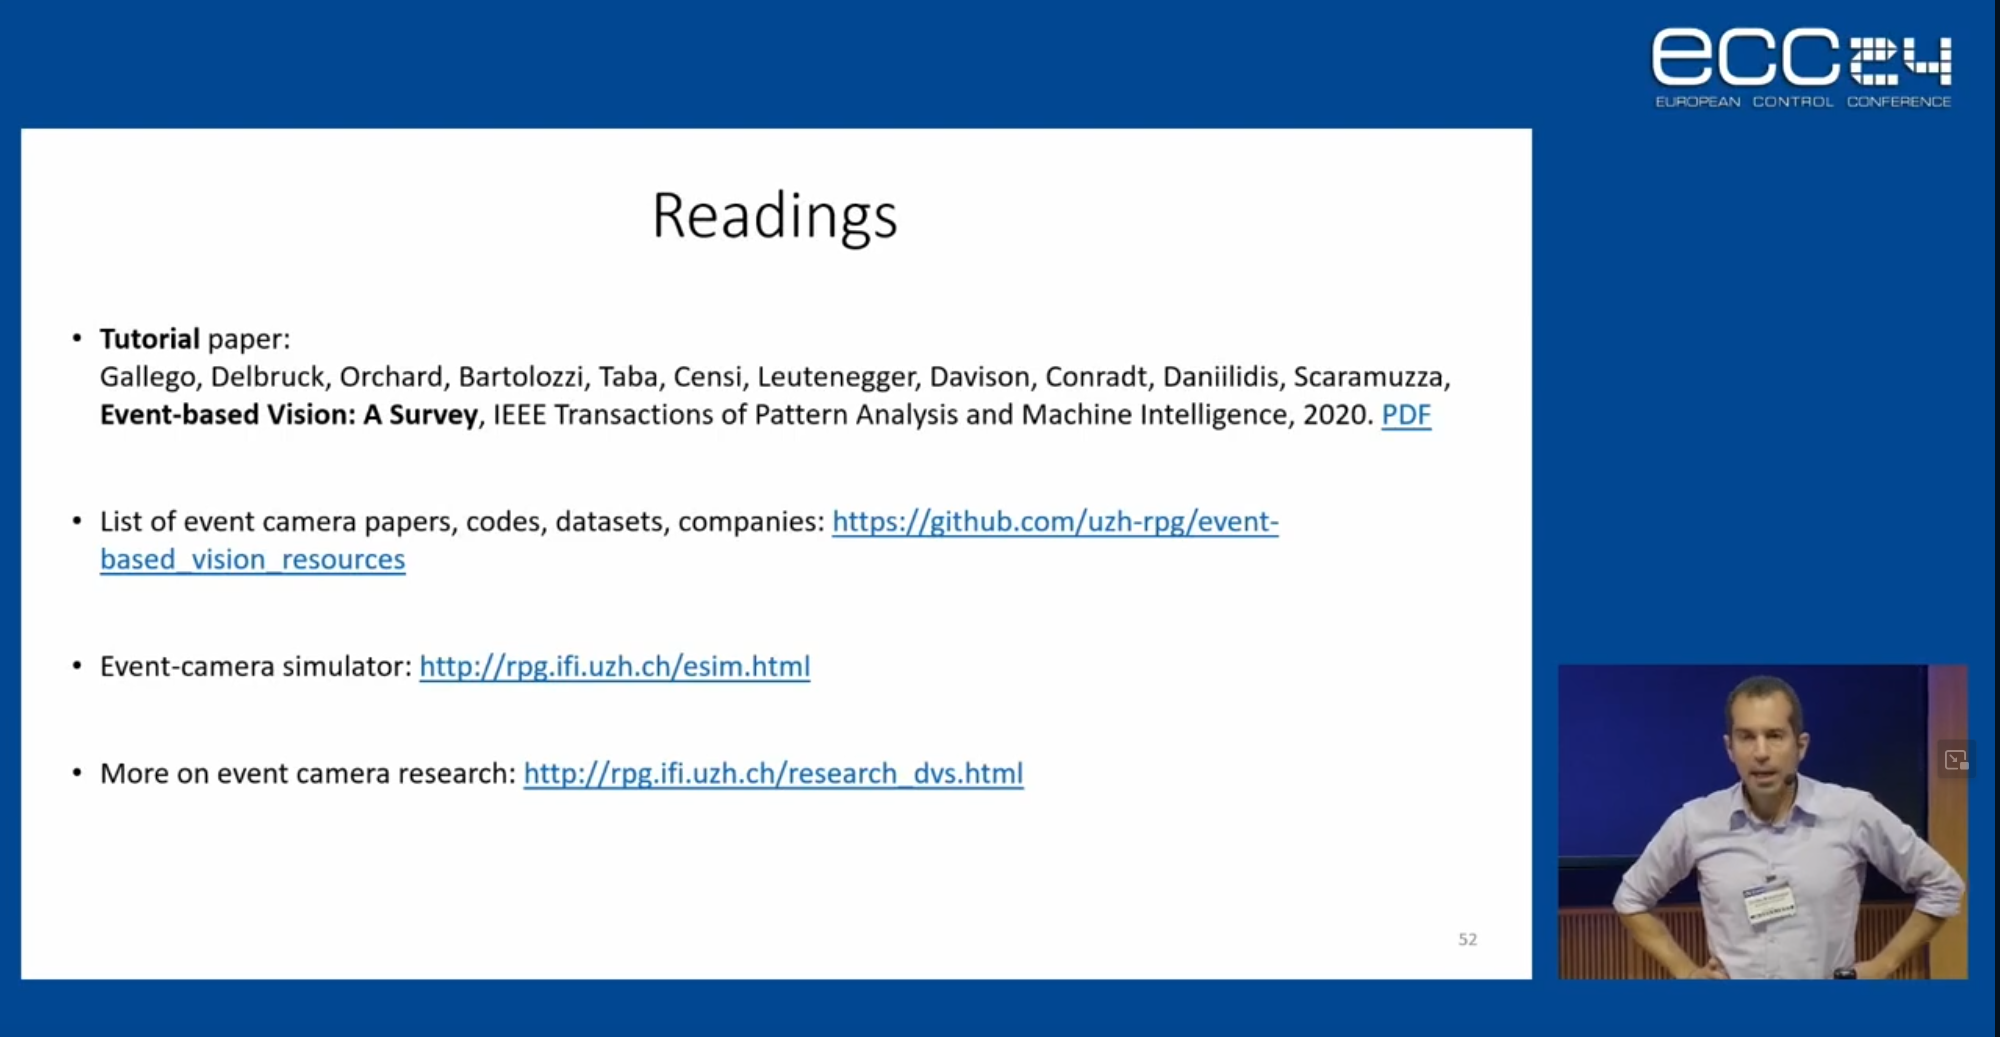
\includegraphics[width=0.8\textwidth]{assets/reading-list.png}
        \caption{Reading List for Event Cameras and Robotics}
        \label{fig:reading_list}
    \end{figure}

    ?? CAN WE USE EVENT CAMERAS TO HELP LAND A HELICOPTER IF THE ENGINE FAILES??
    

\end{itemize}

\section{Robert Mahony}
Australian National University.
\\Systems Theory and Robotics group.
\\Austarlia


\section{Interesting Papers and Works}

\subsection{Guido de Croon - MAVLAB}
    \begin{itemize}
        \item \textit{[4] Guido de Croon et al., MAVRL: Learn to Fly in Cluttered Environments with Varying Speed \href{https://arxiv.org/abs/2402.08381}{arXiv:2402.08381}}
        \begin{itemize}
            \item They show that they a RL method to train obstacle avoidance in cluttered environments (forests), 
                  They claim their path planning model doesn't rely on constant high speed. Making it better for both safety
                  and agility in complex environments.
        \end{itemize}
        \item They also provide a simulator (I think it is based on \textbf{Agiluis platform from Davide Scaramuzza})
                They use the simulator to benchmark obstacle avoidance \textit{\textbf{AvoidBench}} \href{https://mavlab.tudelft.nl/avoidbench-icra-2023/}{https://mavlab.tudelft.nl/avoidbench-icra-2023/} 
        
        \begin{figure}[H]
            \centering
            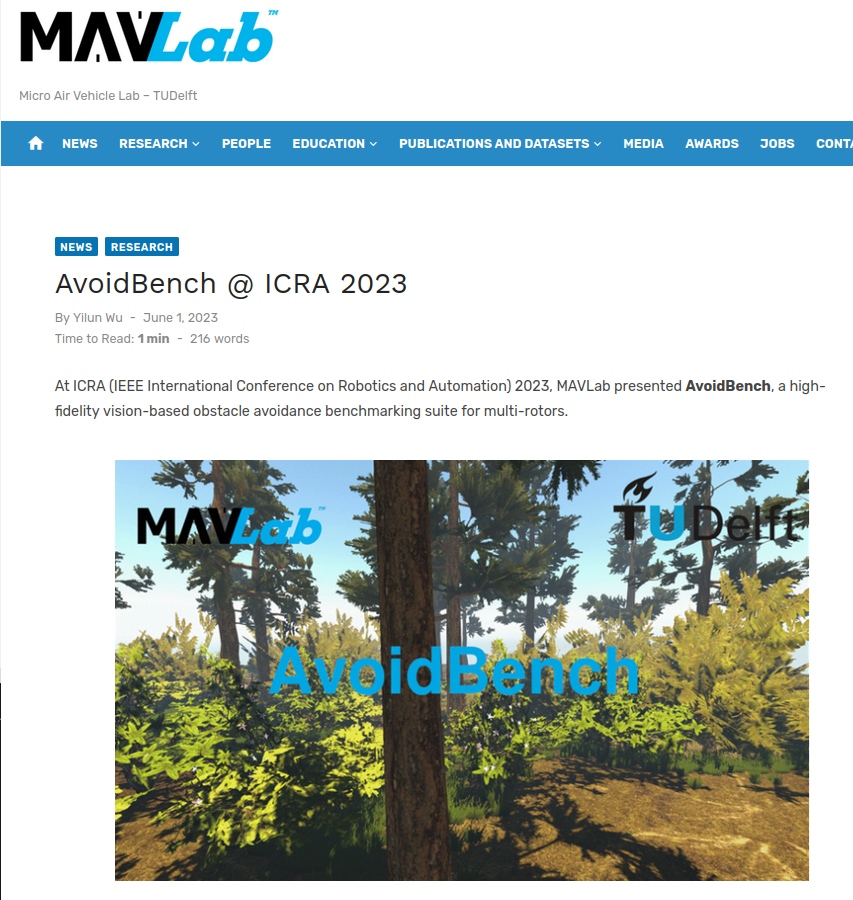
\includegraphics[width=0.8\textwidth]{assets/mavlab-avoid-bench.png}
            \caption{AvoidBench Simulator}
            \label{fig:avoidbench}
        \end{figure}
        
    \end{itemize}

\section{Methodology}
We propose...

\section{Resources}
\begin{itemize}
    \item Event-based Vision Resources (link): \href{https://github.com/uzh-rpg/event-based_vision_resources?tab=readme-ov-file#event-based-vision-resources}{GitHub Repository}
\end{itemize}

\section{Conclusion}
This approach...


\section{Influenctional Papers}

\end{document}
